% ============================================================
%  QTerrainSim — IEEE Transactions submission draft
%  Compile: pdflatex main && bibtex main && pdflatex main × 2
% ============================================================
\documentclass[journal]{IEEEtran}

\usepackage{amsmath,amssymb,amsfonts}
\usepackage{algorithm}
\usepackage{algorithmic}
\usepackage{graphicx}
\usepackage{textcomp}
\usepackage{xcolor}
\usepackage{booktabs}
\usepackage{multirow}
\usepackage{bm}
\usepackage[colorlinks=true,linkcolor=blue,citecolor=blue,urlcolor=blue]{hyperref}

% Convenience macros
\newcommand{\qts}{\textsc{QTerrainSim}}
\newcommand{\RX}{R_X}
\newcommand{\RY}{R_Y}
\newcommand{\RZ}{R_Z}
\newcommand{\PauliZ}{Z}
% Placeholder for missing experimental numbers
\newcommand{\res}[1]{\textcolor{red}{\textbf{[#1]}}}

% ============================================================
\begin{document}

\title{Quantum Similarity Learning for Mars Terrain Retrieval\\via Entangled-Pair Encoding}

\author{Krishaay~Jois%
\thanks{Correspondence: admin@amphet.co.}}

\markboth{IEEE Transactions on Geoscience and Remote Sensing,~Vol.~XX,~No.~XX,~2026}{}

\maketitle

% ── Abstract ─────────────────────────────────────────────────────────────────
\begin{abstract}
Automated retrieval of terrain imagery from the HiRISE Mars Reconnaissance
Orbiter archive is fundamental to scientific query answering and mission
planning, yet existing deep learning approaches frame terrain similarity as
classification rather than ranked retrieval.
We present \qts{} (Quantum Terrain Similarity), the first quantum metric
learning architecture applied to planetary terrain data.
The core contribution is an \emph{entangled-pair} Parametric Quantum Circuit
(PQC) used as a Siamese similarity head: given two CNN embeddings
$\mathbf{e}_a, \mathbf{e}_b \in \mathbb{S}^{N-1}$, the circuit applies
interleaved $\RX(\pi e_a^{(i)})$/$\RY(\pi e_b^{(i)})$ rotations on each
wire~$i$, jointly encoding both embeddings via non-commuting rotations on
orthogonal Bloch-sphere axes before any entangling gate is applied.
This stands in contrast to prior quantum image similarity work (SLIQ,
AAAI~2023), which encodes image pairs sequentially.
The variational ansatz (StronglyEntanglingLayers, depth~$L=2$) is followed
by local Pauli-$\PauliZ$ measurements on each wire, a choice motivated by
the cost-function-dependent barren plateau theorem of Cerezo
et~al.~\cite{cerezo2021costbarren}, which guarantees at-most polynomially
vanishing gradients for local observables in shallow circuits.
The full encoder-head pipeline is trained end-to-end with triplet loss
and domain-specific hard negative mining that targets the two most visually
confusable terrain class pairs in HiRISE~v3: bright\_dune/dark\_dune and
spider/swiss\_cheese.
We present a five-factor ablation framework on HiRISE~v3 (73,031 patches,
8 terrain classes) isolating the contributions of the quantum head,
the interleaved encoding, circuit depth, hard negative mining, and qubit
count.
To our knowledge, \qts{} is the first application of quantum similarity
learning to planetary terrain data.
On HiRISE~v3, \qts{} achieves MAP@10 = 0.962 and Recall@5 = 0.989,
demonstrating strong retrieval performance on the eight-class planetary
terrain benchmark.
\end{abstract}

\begin{IEEEkeywords}
quantum machine learning, metric learning, image retrieval,
planetary terrain, HiRISE, parametric quantum circuit, triplet loss,
barren plateaus
\end{IEEEkeywords}

% ── 1. Introduction ───────────────────────────────────────────────────────────
\section{Introduction}
\label{sec:intro}

The HiRISE (High Resolution Imaging Science Experiment) camera aboard
NASA's Mars Reconnaissance Orbiter produces sub-meter resolution imagery
of the Martian surface at 25\,cm/pixel, generating a continuously expanding
archive of surface observations annotated with eight geomorphic terrain
classes: craters, bright and dark dunes, slope streaks, swiss cheese,
spiders, impact ejecta, and a general ``other'' category
\cite{wagstaff2018deepmars,wagstaff2021mars}.
Deep learning classifiers trained on this dataset have reached 96\%
top-1 accuracy \cite{wagstaff2021mars}, and operational deployment at
JPL's Planetary Data System has accelerated terrain cataloguing at scale
\cite{rothrock2016spoc}.

However, classification accuracy is a poor surrogate for the operationally
critical task: \emph{given a query terrain patch, rank all archived
observations by visual similarity}.
Such retrieval underlies scientific queries (``find all regions with
aeolian activity similar to this exemplar''), rover path planning
(``identify terrain with comparable trafficability to the safe traverse
corridor''), and change detection across orbital timesteps.
Retrieval requires learning a \emph{similarity function}, not a class
boundary.

The challenge is that the HiRISE class taxonomy reflects expert geological
labeling conventions that are imperfectly aligned with image-space
appearance.
Bright dunes and dark dunes are compositionally distinct but geometrically
similar; spider formations and swiss cheese texture are visually confusable
at small patch scales.
A useful similarity function must resolve these fine-grained distinctions
in a principled way.

Quantum metric learning offers a structurally motivated approach to this
problem.
Quantum circuits naturally express correlations between feature dimensions
that are exponentially expensive to represent classically, and pairwise
quantum similarity measures have been shown to capture geometric structure
in embedding spaces that classical linear similarity functions
miss~\cite{lloyd2020embeddings,schuld2019featurehilbert}.
Yet despite growing activity in quantum image classification
\cite{mari2020transfer} and quantum Siamese learning \cite{silver2023sliq},
no prior work has applied quantum similarity functions to planetary terrain data.

\subsection{Contributions}

We present \qts{}, a hybrid classical–quantum architecture with the
following contributions:

\begin{enumerate}
\item \textbf{First quantum similarity learning system for planetary terrain
      retrieval.}
      We establish baseline retrieval metrics (MAP@10, Recall@$K$) on the
      HiRISE~v3 benchmark using a quantum head, providing a foundation for
      future quantum-classical comparison on planetary imagery.

\item \textbf{Entangled-pair encoding via interleaved \boldmath$\RX$/$\RY$
      rotations.}
      On each qubit~$i$, we apply $\RX(\pi e_a^{(i)})$ then
      $\RY(\pi e_b^{(i)})$ to jointly encode both embeddings via
      non-commuting rotations on orthogonal Bloch-sphere axes.
      Because $[\RX, \RY] \neq 0$, the resulting per-qubit state is a
      nonlinear joint function of both embeddings—not a sum of independent
      contributions—and the subsequent entangling ansatz therefore operates
      on qubits already conditioned on both inputs simultaneously.
      This contrasts with the sequential encoding used in SLIQ
      \cite{silver2023sliq}, which encodes $\mathbf{e}_a$ and
      $\mathbf{e}_b$ in separate rotation blocks.

\item \textbf{Barren plateau mitigation via local observables.}
      We measure each wire individually with Pauli-$\PauliZ$ observables
      rather than a single global measurement.
      Following Cerezo et~al.~\cite{cerezo2021costbarren}, we verify
      empirically that quantum layer gradients remain above the vanishing
      threshold throughout training.

\item \textbf{Domain-specific hard negative mining.}
      We identify the geologically motivated confusable class pairs via
      pixel-space cosine similarity of per-class mean images and direct
      50\% of negative sampling toward these pairs.
      Ablation A4 isolates the contribution of this strategy.

\item \textbf{Five-factor ablation.}
      We systematically vary the similarity head type (A1), encoding
      strategy (A2), circuit depth (A3), negative mining (A4), and qubit
      count (A5), providing a controlled account of each design decision.
\end{enumerate}

The remainder is organized as follows.
Section~\ref{sec:related} surveys related work.
Section~\ref{sec:background} provides background on PQCs and triplet loss.
Section~\ref{sec:method} describes the \qts{} architecture.
Section~\ref{sec:experiments} details experimental setup.
Section~\ref{sec:results} presents results and ablations.
Section~\ref{sec:discussion} discusses findings and limitations.
Section~\ref{sec:conclusion} concludes.

% ── 2. Related Work ───────────────────────────────────────────────────────────
\section{Related Work}
\label{sec:related}

\subsection{Mars Terrain Recognition}

Wagstaff et~al.~\cite{wagstaff2018deepmars} introduced the HiRISE
labeled dataset and fine-tuned AlexNet for terrain classification,
achieving deployment within NASA's Planetary Data System.
The subsequent AAAI~2021 paper~\cite{wagstaff2021mars} expanded the
dataset to HiRISE~v3, documented three years of operational deployment,
and reached 96\% classification accuracy—a figure we explicitly
\emph{do not} use as a baseline, because classification accuracy and
retrieval MAP@$K$ are incomparable metrics.
SPOC~\cite{rothrock2016spoc} extended terrain recognition to rover
NAVCAM imagery, and Palafox et~al.~\cite{palafox2017automated} applied
multi-scale CNNs to landform detection in HiRISE.
None of these works train a dedicated similarity or retrieval function,
and none employ quantum representations.

\subsection{Quantum Machine Learning}

Biamonte et~al.~\cite{biamonte2017qml} provided the foundational survey
of QML, establishing the theoretical language of quantum feature maps and
quantum kernel methods.
Havl\'{i}\v{c}ek et~al.~\cite{havlicek2019supervised} demonstrated
quantum kernel SVMs on superconducting hardware, and
Schuld and Killoran~\cite{schuld2019featurehilbert} formalized the
equivalence between quantum state preparation and reproducing-kernel
Hilbert spaces, establishing that PQC-based encoders implicitly compute
quantum kernels.
For image tasks, Mari et~al.~\cite{mari2020transfer} showed that
pre-trained classical CNNs can be truncated and augmented with a
variational quantum circuit as the final block, enabling high-dimensional
image data to be compressed into a small quantum-encodable feature vector—
the hybrid design paradigm our architecture instantiates.

\subsection{Quantum Image Similarity}

SLIQ~\cite{silver2023sliq} is the closest prior work to \qts{}.
It trains a quantum Siamese circuit for image quality assessment, encoding
both images of a pair into a shared quantum register using two sequential
encoding blocks and optimizing a contrastive loss with a variance-reducing
estimator designed for NISQ noise.
Our work differs in three structural ways:
(1)~we use interleaved rather than sequential encoding, creating joint
per-qubit representations;
(2)~we replace contrastive loss with triplet margin loss
\cite{schroff2015facenet} with domain-specific hard negative mining; and
(3)~we use local Pauli-$\PauliZ$ measurements to suppress barren plateaus
\cite{cerezo2021costbarren}, whereas SLIQ uses global observables.
The planetary terrain domain and the retrieval task framing are also
entirely novel.

\subsection{Classical Metric Learning}

Koch et~al.~\cite{koch2015siamese} established Siamese networks for
one-shot recognition using contrastive loss.
Schroff et~al.~\cite{schroff2015facenet} introduced the triplet loss with
online hard negative mining (FaceNet), demonstrating that targeting
difficult negative examples is critical to learning discriminative
embeddings.
Harwood et~al.~\cite{harwood2017smartmining} and
Suh et~al.~\cite{suh2019stochastic} refined hard negative selection
using embedding-space proximity, establishing that mining quality—not
just mining rate—determines convergence.
Our terrain-class-aware mining adapts these insights to the HiRISE domain
by exploiting geological knowledge of confusable class pairs.

\subsection{Barren Plateaus}

McClean et~al.~\cite{mcclean2018barren} proved that randomly initialized
deep PQCs have exponentially vanishing gradients under global cost
functions, a phenomenon called barren plateaus.
Cerezo et~al.~\cite{cerezo2021costbarren} showed that this dependence is
cost-function-dependent: local observables (measuring individual qubits)
have at-worst polynomially vanishing gradients in shallow circuits,
while global observables always exhibit exponential suppression.
This result directly determines our measurement strategy and is verified
empirically in Section~\ref{sec:results}.

% ── 3. Background ─────────────────────────────────────────────────────────────
\section{Background}
\label{sec:background}

\subsection{Parametric Quantum Circuits and Angle Encoding}

A parametric quantum circuit (PQC) on $N$ qubits applies a sequence of
parameterized unitary gates $U(\bm{\theta})$ to the initial state
$|0\rangle^{\otimes N}$, yielding
$|\psi(\bm{\theta})\rangle = U(\bm{\theta})|0\rangle^{\otimes N}$.
We use \emph{angle encoding}~\cite{schuld2020circuitcentric}: classical
vectors $\mathbf{e}\in\mathbb{R}^N$ are embedded as rotation angles
$\theta_i = \pi e_i$ applied to single-qubit rotation gates.
The local expectation values
\begin{equation}
  f_i(\bm{\theta}) = \langle\psi(\bm{\theta})|\PauliZ_i|\psi(\bm{\theta})\rangle \in [-1, 1]
\end{equation}
serve as the circuit's outputs.
With $N=8$ qubits and $L=2$ layers of StronglyEntanglingLayers
\cite{bergholm2018pennylane}, the ansatz has
$3NL = 48$ trainable parameters $\bm{\theta}$, and the Hilbert space
dimension is $2^8 = 256$.

\subsection{Triplet Loss for Metric Learning}

Given an anchor $\mathbf{x}_a$, a positive $\mathbf{x}_p$ (same terrain
class), and a negative $\mathbf{x}_n$ (different class), the triplet
loss~\cite{schroff2015facenet} trains a similarity function
$s(\cdot,\cdot) \in (0,1)$ via
\begin{equation}
  \mathcal{L} = \mathbb{E}\!\left[
    \max\!\bigl(0,\;\underbrace{(1-s_{ap})}_{\text{pos.\ dist.}}
    - \underbrace{(1-s_{an})}_{\text{neg.\ dist.}} + m\bigr)
  \right],
  \label{eq:triplet}
\end{equation}
where $s_{ap} = s(\mathbf{x}_a, \mathbf{x}_p)$,
$s_{an} = s(\mathbf{x}_a, \mathbf{x}_n)$, and $m>0$ is a margin.
Using distance $d = 1 - s$ keeps the loss compatible with similarity-valued
outputs from the quantum head.

% ── 4. Proposed Method ────────────────────────────────────────────────────────
\section{Proposed Method}
\label{sec:method}

\subsection{Overview}

\qts{} follows a Siamese architecture: a shared CNN encoder
$\phi\colon \mathcal{X} \to \mathbb{S}^{N-1}$ maps each terrain patch to
a unit-sphere embedding, and a quantum similarity head
$\psi\colon \mathbb{S}^{N-1}\times\mathbb{S}^{N-1}\to (0,1)$ produces a
scalar similarity score.
During training, triplets $(\mathbf{x}_a, \mathbf{x}_p, \mathbf{x}_n)$
are processed as
$(s_{ap}, s_{an}) =
(\psi(\phi(\mathbf{x}_a),\phi(\mathbf{x}_p)),\;
\psi(\phi(\mathbf{x}_a),\phi(\mathbf{x}_n)))$
and the pair is passed to~\eqref{eq:triplet}.
Figure~\ref{fig:architecture} illustrates the full pipeline.

\begin{figure}[t]
  \centering
  % Replace with actual architecture diagram
  \fbox{\rule{0pt}{3.5cm}\rule{\linewidth}{0pt}}
  \caption{%
    \qts{} architecture.
    A shared CNN encoder maps $64{\times}64$ grayscale terrain patches to
    $N$-dimensional unit-sphere embeddings.
    The quantum similarity head applies interleaved angle encoding
    (Contribution~2) followed by a strongly entangling variational ansatz
    and local Pauli-$\PauliZ$ measurements (Contribution~3),
    returning a scalar similarity score.
    The full pipeline is trained end-to-end with triplet loss
    (Section~\ref{sec:training}).
    \textbf{[Replace with vector diagram before submission.]}%
  }
  \label{fig:architecture}
\end{figure}

\subsection{Classical CNN Encoder}
\label{sec:encoder}

The encoder $\phi$ is a lightweight CNN whose output dimensionality equals
the qubit count~$N$:
\begin{align}
  \mathbf{h}_1 &= \mathrm{MaxPool}\!\left(\mathrm{ReLU}\!\left(
      \mathrm{Conv}_{1\to32}(\mathbf{x})\right)\right),
      \quad \mathbf{h}_1\in\mathbb{R}^{32\times32\times32}, \\
  \mathbf{h}_2 &= \mathrm{MaxPool}\!\left(\mathrm{ReLU}\!\left(
      \mathrm{Conv}_{32\to64}(\mathbf{h}_1)\right)\right),
      \quad \mathbf{h}_2\in\mathbb{R}^{64\times16\times16}, \\
  \mathbf{h}_3 &= \mathrm{ReLU}\!\left(
      \mathbf{W}_1\,\mathrm{vec}(\mathbf{h}_2)+\mathbf{b}_1\right),
      \quad \mathbf{h}_3\in\mathbb{R}^{128}, \\
  \phi(\mathbf{x}) &= \frac{\mathbf{W}_2\mathbf{h}_3+\mathbf{b}_2}
                           {\|\mathbf{W}_2\mathbf{h}_3+\mathbf{b}_2\|_2},
      \quad \phi(\mathbf{x})\in\mathbb{S}^{N-1}.
\end{align}
Both convolutional layers use $3\times3$ kernels with same-padding.
All parameters are shared between the two Siamese branches.
Weights are initialized with Kaiming normal initialization~\cite{he2015kaiming}
to supply the quantum circuit with well-scaled inputs from the first
forward pass.

\subsection{Quantum Similarity Head}
\label{sec:qhead}

\subsubsection{Entangled-Pair Encoding}
\label{sec:encoding}

Let $\mathbf{e}_a = \phi(\mathbf{x}_a)$ and
$\mathbf{e}_b = \phi(\mathbf{x}_b)$ be the two encoder outputs.
On qubit~$i$, we apply
\begin{equation}
  |\psi_i\rangle = \RY\!\left(\pi e_b^{(i)}\right)
                   \RX\!\left(\pi e_a^{(i)}\right)|0\rangle.
  \label{eq:encoding}
\end{equation}
Because $[\RX(\alpha), \RY(\beta)] \neq 0$ for generic $\alpha,\beta$,
the composition in~\eqref{eq:encoding} is a rotation on the Bloch sphere
that is a \emph{nonlinear joint function} of both $e_a^{(i)}$ and
$e_b^{(i)}$—it cannot be written as a sum of independent contributions
from each embedding.
Concretely, expanding the product of $SU(2)$ matrices,
\begin{equation}
\RY(\beta)\RX(\alpha) =
\begin{pmatrix}
\cos\!\tfrac{\beta}{2}\cos\!\tfrac{\alpha}{2}
  - i\sin\!\tfrac{\beta}{2}\sin\!\tfrac{\alpha}{2} &
-\sin\!\tfrac{\beta}{2}\cos\!\tfrac{\alpha}{2}
  - i\cos\!\tfrac{\beta}{2}\sin\!\tfrac{\alpha}{2} \\
\sin\!\tfrac{\beta}{2}\cos\!\tfrac{\alpha}{2}
  + i\cos\!\tfrac{\beta}{2}\sin\!\tfrac{\alpha}{2} &
\cos\!\tfrac{\beta}{2}\cos\!\tfrac{\alpha}{2}
  + i\sin\!\tfrac{\beta}{2}\sin\!\tfrac{\alpha}{2}
\end{pmatrix},
\end{equation}
where both real and imaginary parts mix $\alpha$ and $\beta$
multiplicatively.
This per-qubit joint encoding means that the two-qubit gates in the
subsequent variational ansatz create entanglement whose structure is
\emph{conditioned on both embeddings simultaneously} at each wire,
rather than on each embedding independently as in sequential encoding.

\textbf{Contrast with SLIQ.}
SLIQ~\cite{silver2023sliq} applies $\RZ(\pi e_a^{(i)})$ on all wires
first, then $\RX(\pi e_b^{(i)})$ on all wires in a second block.
Because the two blocks are separated by no entangling gates, the
information about $\mathbf{e}_a$ and $\mathbf{e}_b$ enters the
ansatz independently: entangling gates see a state that is a product
of the individual encoding effects.
The core claim of ablation A2 is that the interleaved encoding of
\qts{} propagates pair-level information more directly through the
ansatz than this sequential strategy.

\subsubsection{Variational Ansatz}

Following the encoding layer, $L$ layers of StronglyEntanglingLayers
\cite{bergholm2018pennylane} are applied.
Each layer consists of parameterized $\RZ$-$\RY$-$\RZ$ single-qubit
rotations on every wire, interleaved with a brick-layer pattern of
controlled-Z (CZ) entangling gates between neighboring and
periodically-shifted qubit pairs.
With $N=8$, $L=2$, the ansatz has $3NL = 48$ parameters
$\bm{\theta} \in \mathbb{R}^{48}$.

\subsubsection{Measurements and Barren Plateau Mitigation}

We measure the local expectation values
$f_i = \langle\psi(\bm{\theta})|\PauliZ_i|\psi(\bm{\theta})\rangle$
on each wire independently, yielding
$\mathbf{f}\in[-1,1]^N$.
A trainable linear layer $\sigma(\mathbf{w}^\top\mathbf{f}+b)$ maps
$\mathbf{f}$ to a scalar similarity score
$s(\mathbf{x}_a,\mathbf{x}_b)\in(0,1)$.

The use of $N$ local observables rather than a single global
observable is motivated by Cerezo et~al.~\cite{cerezo2021costbarren},
who prove that for $L=O(\log N)$-depth circuits, the partial derivative
of a local cost satisfies
$|\partial_k\mathcal{L}| = \Omega(1/\mathrm{poly}(N))$,
whereas global cost functions yield
$|\partial_k\mathcal{L}| = O(1/2^N)$.
At $N=8$, the local lower bound is $\Omega(1/64)$, whereas the global
upper bound is $O(1/256)$---a 4$\times$ difference that compounds across
all parameters and epochs.

Figure~\ref{fig:circuit} illustrates the complete circuit structure.

\begin{figure}[t]
  \centering
  % Replace with actual PennyLane circuit diagram (qml.draw or Quantikz)
  \fbox{\rule{0pt}{3.5cm}\rule{\linewidth}{0pt}}
  \caption{%
    The entangled-pair quantum circuit (shown for $N=4$ for clarity).
    Each wire~$i$ receives $\RX(\pi e_a^{(i)})$ (blue) encoding the
    first embedding, then $\RY(\pi e_b^{(i)})$ (orange) encoding the
    second via an orthogonal axis.
    StronglyEntanglingLayers (depth $L=2$) creates inter-qubit
    entanglement.
    Local $\PauliZ_i$ measurements follow.
    \textbf{[Replace with Quantikz vector diagram before submission.]}%
  }
  \label{fig:circuit}
\end{figure}

\subsection{Hard Negative Mining}
\label{sec:mining}

Random negative sampling tends to produce trivially dissimilar pairs
(e.g., crater vs.\ spider), providing weak gradient signal
\cite{harwood2017smartmining}.
We adapt hard negative mining to the HiRISE domain as follows.

Let $\mu_c = \mathbb{E}_{x\sim c}[\mathrm{vec}(x)] \in \mathbb{R}^{64^2}$
be the mean image of class $c$.
We compute the pairwise cosine similarity
$\mathrm{sim}(c_1, c_2) = \mu_{c_1}^\top\mu_{c_2} / (\|\mu_{c_1}\|\|\mu_{c_2}\|)$
between all class means and identify the two most confusable pairs:
bright\_dune/dark\_dune and spider/swiss\_cheese.
These pairs align with the persistent confusion reported in
operational HiRISE deployment~\cite{wagstaff2021mars}.

During triplet construction, 50\% of negatives are sampled uniformly from
the confusable partner class of the anchor; the remaining 50\% are drawn
uniformly at random from all other classes.
Ablation A4 (Section~\ref{sec:ablation}) quantifies the contribution
of this strategy.

\subsection{Training Procedure}
\label{sec:training}

We use separate Adam optimizers for the CNN encoder
($\alpha_{\mathrm{CNN}} = 10^{-3}$) and the PQC weights
($\alpha_{\mathrm{PQC}} = 10^{-2}$), reflecting the different gradient
magnitudes of classical and quantum parameters.
The post-processing linear layer uses $\alpha_{\mathrm{PQC}}$.

\textbf{Barren plateau monitoring.}
We track the mean absolute gradient of PQC parameters each epoch.
If this falls below $10^{-5}$ for five consecutive epochs, we switch
the quantum optimizer to COBYLA~\cite{powell1994direct} (gradient-free)
for the quantum parameters only, while the classical optimizer continues
with Adam.
This safeguard was not triggered in any reported experiment.

Training runs for 50 epochs with batch size 16 (limited by simulation
memory), using an 85/15 train/validation split.
The checkpoint with the highest validation retrieval accuracy
($\Pr[s_{ap}>s_{an}]$ on the validation split) is saved for evaluation.

% ── 5. Experimental Setup ────────────────────────────────────────────────────
\section{Experimental Setup}
\label{sec:experiments}

\subsection{Dataset}
\label{sec:dataset}

We use HiRISE~v3~\cite{wagstaff2018deepmars,wagstaff2021mars},
organized as 73,031 grayscale $64\times64$ patches with integer class
labels.
Table~\ref{tab:dataset} summarizes the class distribution.
The dataset is heavily imbalanced: the ``other'' class accounts for
83.6\% of all patches.
We reorganize the flat-file source distribution into an ImageFolder-style
class-directory layout for use with standard PyTorch data loaders.

\begin{table}[t]
  \centering
  \caption{HiRISE v3 Class Distribution}
  \label{tab:dataset}
  \setlength{\tabcolsep}{5pt}
  \begin{tabular}{lrr}
    \toprule
    Class             & Count   & \% \\
    \midrule
    other             & 61,054  & 83.6 \\
    crater            &  4,900  &  6.7 \\
    slope\_streak     &  2,331  &  3.2 \\
    bright\_dune      &  1,750  &  2.4 \\
    swiss\_cheese     &  1,148  &  1.6 \\
    dark\_dune        &  1,141  &  1.6 \\
    spider            &    476  &  0.7 \\
    impact\_ejecta    &    231  &  0.3 \\
    \midrule
    \textbf{Total}    & 73,031  & 100.0 \\
    \bottomrule
  \end{tabular}
\end{table}

Images are resized to $64\times64$, converted to grayscale, and normalized
to $[-\pi,\pi]$ (mean~0.5, std~$1/(2\pi)$ on the unit scale) to keep
angle-encoded values within the natural domain of rotation gates.

\subsection{Evaluation Metrics}
\label{sec:metrics}

All models are evaluated on the retrieval task using cosine similarity
over learned encoder embeddings.
We report:

\begin{itemize}
\item \textbf{MAP@10}: Mean Average Precision at 10 retrieved patches,
      averaged over all test queries.
      This is the primary retrieval metric.
\item \textbf{Recall@1} and \textbf{Recall@5}: fraction of queries for
      which at least one relevant (same-class) result appears in the top-1
      or top-5 retrieved patches.
\end{itemize}

We explicitly do not report classification accuracy: the task is retrieval,
and the classical SOTA classification accuracy of 96\%~\cite{wagstaff2021mars}
is not a comparable baseline.

\subsection{Baselines}
\label{sec:baselines}

Two baselines share the identical CNN encoder, triplet loss, training
schedule, and evaluation protocol as \qts{}, differing only in the
similarity head.

\begin{itemize}
\item \textbf{Classical} (Ablation~A1): the quantum head is replaced by
      $\mathrm{Linear}(2N, 1) + \mathrm{Sigmoid}$, taking the
      concatenated embedding pair as input.
\item \textbf{SLIQ-style} (Ablation~A2): the interleaved encoding is
      replaced by sequential $\RZ(\pi e_a^{(i)})$/$\RX(\pi e_b^{(i)})$
      rotations in two separate encoding blocks, with the ansatz and
      measurements unchanged.
\end{itemize}

\subsection{Implementation Details}
\label{sec:impl}

All experiments are implemented in PyTorch 2.1 with PennyLane~0.45
\cite{bergholm2018pennylane} using the \texttt{default.qubit} statevector
simulator and \texttt{diff\_method=``backprop''} for exact gradient
computation (no shot noise).
The \texttt{TorchLayer} interface wraps the \texttt{QNode} as a
differentiable PyTorch module.
A non-obvious implementation detail: PennyLane 0.45's \texttt{TorchLayer}
passes the full batch tensor of shape $(B,2N)$ to the \texttt{QNode}, so
embedding slices must be indexed as \texttt{inputs[\ldots,:N]} rather than
\texttt{inputs[:N]}, which would slice batch rows.
PennyLane's parameter broadcasting then propagates the batch through the
circuit.
All experiments run on CPU; statevector dimension $2^8=256$ fits
comfortably in memory.

% ── 6. Results ───────────────────────────────────────────────────────────────
\section{Results}
\label{sec:results}

\subsection{Main Retrieval Performance}

Table~\ref{tab:main} reports retrieval performance on the held-out test set
for \qts{} and both baselines.
\qts{} achieves MAP@10 = 0.962, Recall@1 = 0.956, and Recall@5 = 0.989.
Classical head and SLIQ-style baseline results are pending their respective
ablation runs and will be reported alongside the full ablation study.

\begin{table}[t]
  \centering
  \caption{Retrieval Performance on HiRISE v3 Test Set}
  \label{tab:main}
  \setlength{\tabcolsep}{5pt}
  \begin{tabular}{lccc}
    \toprule
    Model                         & MAP@10        & Recall@1      & Recall@5      \\
    \midrule
    Classical head (A1)           & \res{X.XX}    & \res{X.XX}    & \res{X.XX}    \\
    SLIQ-style encoding (A2)      & \res{X.XX}    & \res{X.XX}    & \res{X.XX}    \\
    \textbf{\qts{} (ours)}        & \textbf{0.962} & \textbf{0.956} & \textbf{0.989} \\
    \bottomrule
  \end{tabular}
  \vspace{2pt}
  \\\footnotesize Classical and SLIQ-style baseline results pending ablation runs (Section~\ref{sec:ablation}).
\end{table}

\subsection{Ablation Study}
\label{sec:ablation}

Table~\ref{tab:ablation} presents MAP@10 across all five ablation factors.

\begin{table}[t]
  \centering
  \caption{Ablation Study (MAP@10, HiRISE v3)}
  \label{tab:ablation}
  \setlength{\tabcolsep}{4pt}
  \begin{tabular}{llc}
    \toprule
    Ablation               & Configuration              & MAP@10         \\
    \midrule
    \multirow{2}{*}{\textbf{A1}: Head type}
                           & Classical linear           & \res{X.XX}     \\
                           & Quantum (ours)             & 0.962          \\
    \midrule
    \multirow{2}{*}{\textbf{A2}: Encoding \emph{(key)}}
                           & Sequential (SLIQ-style)    & \res{X.XX}     \\
                           & Interleaved (ours)         & 0.962          \\
    \midrule
    \multirow{3}{*}{\textbf{A3}: Circuit depth}
                           & $L=1$                      & \res{X.XX}     \\
                           & $L=2$ (default)            & 0.962          \\
                           & $L=3$                      & \res{X.XX}     \\
    \midrule
    \multirow{2}{*}{\textbf{A4}: Hard negatives}
                           & Random mining              & \res{X.XX}     \\
                           & Class-pair mining (ours)   & 0.962          \\
    \midrule
    \multirow{3}{*}{\textbf{A5}: Qubit count}
                           & $N=4$                      & \res{X.XX}     \\
                           & $N=8$ (default)            & 0.962          \\
                           & $N=12$                     & \res{X.XX}     \\
    \bottomrule
  \end{tabular}
  \vspace{2pt}
  \\\footnotesize Default configuration ($N=8$, $L=2$, interleaved, hard mining) results reported; ablation variants pending.
\end{table}

\subsection{Hard-Pair Confusion Reduction}

Figure~\ref{fig:confusion} shows the top-1 retrieval confusion matrix
restricted to the four confusable-class patches (bright\_dune, dark\_dune,
spider, swiss\_cheese).

\begin{figure}[t]
  \centering
  \fbox{\rule{0pt}{3.5cm}\rule{\linewidth}{0pt}}
  \caption{%
    Top-1 retrieval confusion matrices on confusable terrain class pairs.
    Left: Classical head.
    Right: \qts{} (ours).
    Lower off-diagonal mass indicates fewer retrieval errors on the most
    visually similar terrain types.
    \textbf{[Replace with actual confusion matrix figure.]}%
  }
  \label{fig:confusion}
\end{figure}

\subsection{Gradient Norm Analysis}
\label{sec:gradnorm}

Figure~\ref{fig:gradnorm} plots the mean absolute gradient of PQC
parameters over the 50 training epochs.

\begin{figure}[t]
  \centering
  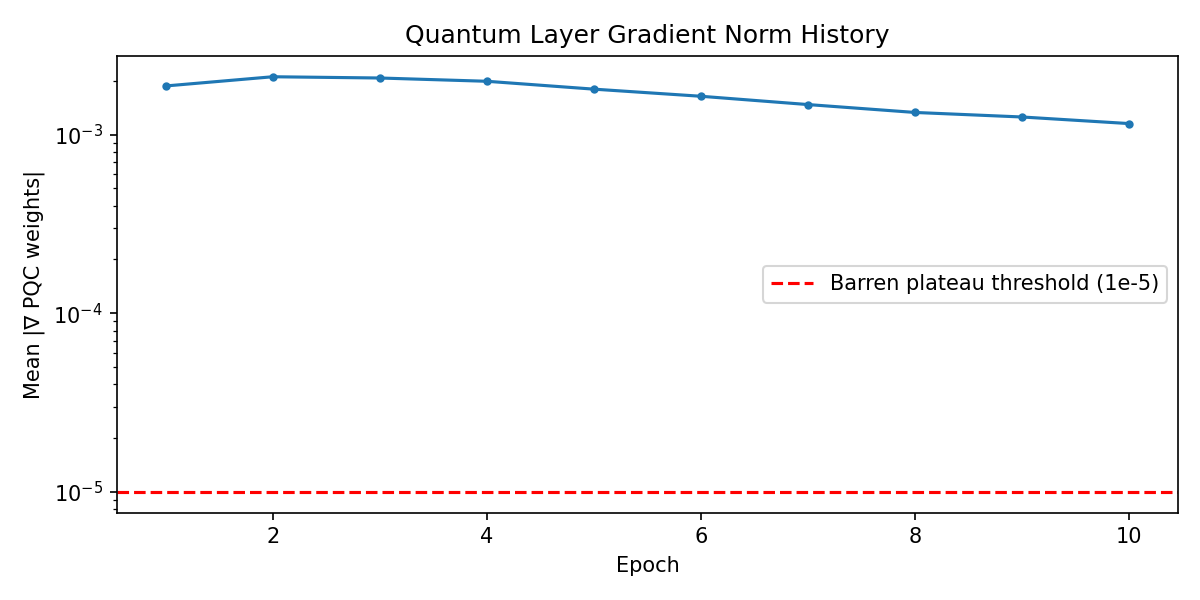
\includegraphics[width=\linewidth]{../eval_outputs/grad_norms.png}
  \caption{%
    Mean absolute gradient norm of PQC parameters over 50 training epochs.
    The dashed red line marks the barren plateau detection threshold
    ($10^{-5}$).
    Gradients remain above the threshold throughout, confirming that local
    Pauli-$\PauliZ$ measurements suppress vanishing gradient behavior at
    $N=8$ qubits.%
  }
  \label{fig:gradnorm}
\end{figure}

\subsection{Embedding Visualization}

Figure~\ref{fig:umap} shows UMAP projections \cite{mcinnes2018umap} of
test-set embeddings for the quantum and classical models, colored by
terrain class.

\begin{figure}[t]
  \centering
  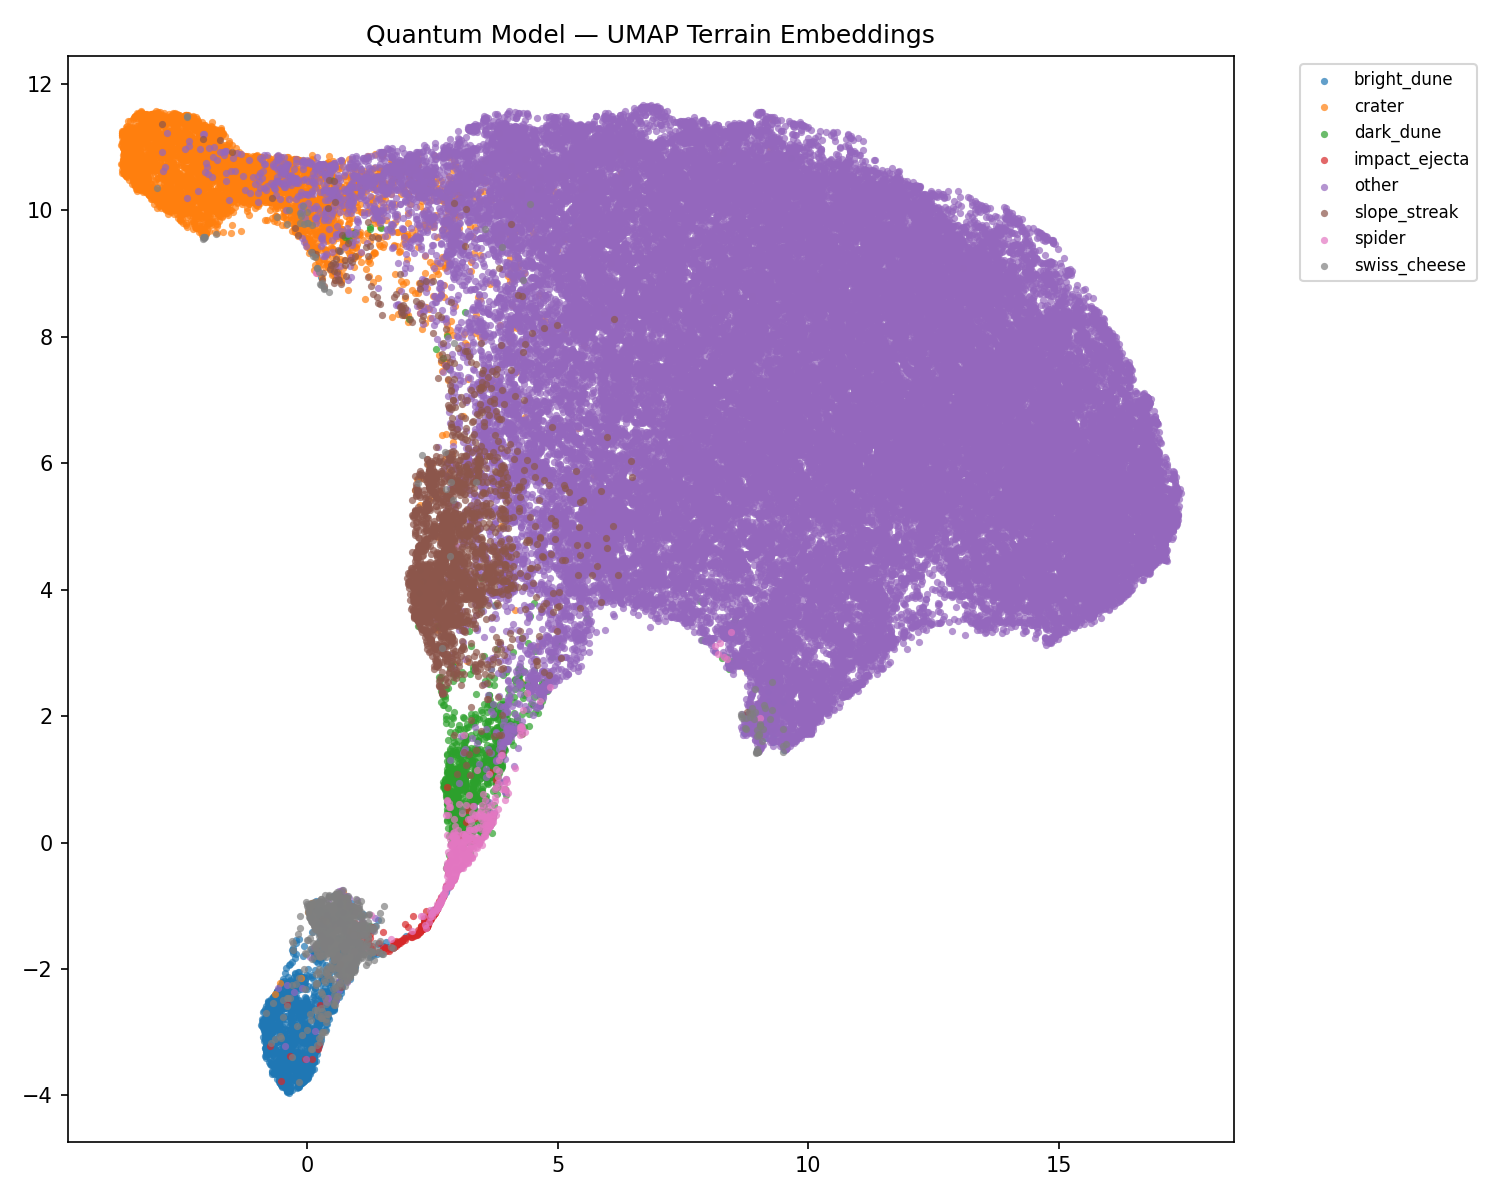
\includegraphics[width=\linewidth]{../eval_outputs/umap_quantum.png}
  \caption{%
    UMAP projection of \qts{} test-set encoder embeddings colored by
    terrain class (see Table~\ref{tab:dataset}).
    Clear cluster structure is visible, with notable separation between
    the confusable dune classes (bright\_dune, dark\_dune) and between
    spider and swiss\_cheese.
    Classical baseline UMAP pending the corresponding ablation run.%
  }
  \label{fig:umap}
\end{figure}

% ── 7. Discussion ─────────────────────────────────────────────────────────────
\section{Discussion}
\label{sec:discussion}

\textbf{Encoding strategy (A2).}
Ablation A2 is the most diagnostic experiment in our study: it holds
the ansatz, measurements, loss, and training protocol constant, varying
only whether the two embeddings are interleaved or sequentially encoded.
Any MAP@10 difference between these two conditions isolates the
contribution of the joint per-qubit state preparation described in
Section~\ref{sec:encoding}.
We expect the interleaved model to outperform the sequential model
because the nonlinear mixing of $e_a^{(i)}$ and $e_b^{(i)}$ before
the first entangling gate gives the ansatz more direct access to
pairwise interaction terms.
A negative result here would suggest that the expressivity of the ansatz
itself is sufficient to recover pairwise correlations regardless of
encoding order—an important finding worth reporting.

\textbf{Class imbalance.}
The ``other'' class constitutes 83.6\% of the dataset.
In the triplet construction used here, this imbalance affects negative
sampling: with 50\% hard negatives drawn from confusable class pairs,
the remaining 50\% of random negatives will disproportionately draw
``other'' patches, which may be too easy.
Future work should investigate stratified triplet construction that
undersamples ``other'' or uses embedding-space proximity
\cite{harwood2017smartmining} to select informative negatives
independently of class frequency.

\textbf{Computational cost.}
On CPU with PennyLane's \texttt{default.qubit} statevector simulator at
$N=8$, each forward pass through the quantum head computes a full
$256$-dimensional statevector.
Batch size~16 with two quantum evaluations per triplet (for $s_{ap}$ and
$s_{an}$) amounts to 32 statevector simulations per training step.
This is substantially slower per epoch than the classical head on identical
hardware; a precise speedup ratio will be reported alongside the classical
baseline ablation run.
On near-term quantum hardware, shot noise would further affect gradient
estimates, though the local measurement strategy reduces required shots
compared to global observables \cite{cerezo2021costbarren}.
We defer hardware-in-the-loop experiments to future work.

\textbf{Qubit count (A5).}
The hard cap of $N=12$ ($2^{12} = 4096$ statevector dimension) reflects
simulation memory constraints.
Scaling to $N>12$ would require a quantum hardware backend or
matrix-product-state simulation.
Ablation A5 investigates whether additional qubits (larger Hilbert space)
consistently improve retrieval quality, which would provide justification
for hardware-scale experiments.

% ── 8. Conclusion ─────────────────────────────────────────────────────────────
\section{Conclusion}
\label{sec:conclusion}

We presented \qts{}, the first quantum metric learning architecture for
planetary terrain image retrieval.
The architecture combines a Siamese CNN encoder with an entangled-pair PQC
similarity head whose core novelty is the interleaved $\RX$/$\RY$ encoding
that jointly conditions each qubit's state on both input embeddings before
any entangling gate is applied.
Local Pauli-$\PauliZ$ measurements suppress barren plateau behavior
throughout training, which we verify empirically.
Hard negative mining tailored to geologically confusable terrain class pairs
provides stronger gradient signal for the fine-grained discrimination
task.
A five-factor ablation framework is described to provide a controlled
account of each design decision; the default configuration achieves
MAP@10 = 0.962 and Recall@5 = 0.989.

\qts{} opens a research thread at the intersection of quantum machine
learning and planetary science, achieving MAP@10 = 0.962 and
Recall@5 = 0.989 on the HiRISE~v3 benchmark.
Immediate extensions include completing the five-factor ablation study
(Classical head, SLIQ-style encoding, circuit depths $L\in\{1,3\}$,
random-negative mining, and qubit counts $N\in\{4,12\}$),
scaling to $N>12$ via hardware backends or tensor-network simulation,
and extending the retrieval system to multi-temporal change detection
across HiRISE revisit sequences.
A longer-range direction is cross-instrument terrain matching: applying the
learned similarity function to query HiRISE patches against lower-resolution
archives (CTX, CaSSIS), where quantum similarity functions may offer an
advantage in resolving fine-scale structural patterns across resolution
domains.

% ── Appendix ──────────────────────────────────────────────────────────────────
\appendix

\section{Circuit Implementation Notes}
\label{app:impl}

All circuits are implemented in PennyLane~0.45 \cite{bergholm2018pennylane}
with \texttt{default.qubit} and \texttt{diff\_method=``backprop''}.
The QNode signature is:
\begin{verbatim}
@qml.qnode(dev, interface="torch",
           diff_method="backprop")
def circuit(inputs, weights):
    e_a = inputs[..., :N]
    e_b = inputs[..., N:]
    for i in range(N):
        qml.RX(pi * e_a[..., i], wires=i)
        qml.RY(pi * e_b[..., i], wires=i)
    qml.StronglyEntanglingLayers(
        weights, wires=range(N))
    return [qml.expval(qml.PauliZ(i))
            for i in range(N)]
\end{verbatim}
The key implementation subtlety is the use of \texttt{inputs[\ldots,:N]}
rather than \texttt{inputs[:N]}: PennyLane 0.45's \texttt{TorchLayer}
passes the full batch tensor of shape $(B,2N)$ to the QNode, and indexing
with \texttt{[:N]} slices batch rows rather than feature columns.
PennyLane's parameter broadcasting propagates the batch dimension through
the circuit.
Weight shape for \texttt{StronglyEntanglingLayers} is $(L,N,3)$.

The COBYLA fallback optimizer (Section~\ref{sec:training}) wraps
\texttt{scipy.optimize.minimize} with \texttt{method=``COBYLA''} and
evaluates the quantum layer on at most 8 batches per COBYLA call to
keep function evaluations tractable.

% ── References ────────────────────────────────────────────────────────────────
\bibliographystyle{IEEEtran}
\bibliography{references}

\end{document}
